\documentclass[12pt,a4paper]{article}

% ---------- Codificación e idioma ----------
\usepackage[utf8]{inputenc}
\usepackage[T1]{fontenc}
\usepackage[spanish,es-noshorthands]{babel}
\usepackage{lmodern}

% ---------- Paquetes útiles ----------
\usepackage[margin=2.5cm]{geometry}
\usepackage{graphicx}
\usepackage{xcolor}
\usepackage{booktabs}
\usepackage{array}
\usepackage{enumitem}
\usepackage{parskip}
\usepackage{verbatim}
\usepackage[hidelinks]{hyperref}
\usepackage{xurl}   % permite cortar las URLs largas para que no se salgan del margen

% Las capturas están en la carpeta capturas/ del repositorio
\graphicspath{{../capturas/}}

% Más holgura al cortar líneas que terminan en nombres de archivo con \texttt
\setlength{\emergencystretch}{3em}

% Los nombres de código (act9\_pipeline.modelos, ...) pueden cortarse después de un guion bajo
\let\guionbajo\_
\renewcommand{\_}{\guionbajo\allowbreak}

% ---------- Referencias con sangria francesa (APA) ----------
\newenvironment{referencias}
  {\begin{list}{}{%
     \setlength{\leftmargin}{1.6em}\setlength{\itemindent}{-1.6em}%
     \setlength{\labelwidth}{0pt}\setlength{\labelsep}{0pt}%
     \setlength{\itemsep}{0.7em}\setlength{\parsep}{0pt}}}
  {\end{list}}

% ---------- Colores ----------
\definecolor{azulUVG}{RGB}{30,90,150}
\definecolor{verde}{RGB}{46,139,87}
\definecolor{grisclaro}{RGB}{240,243,246}
\definecolor{gristexto}{RGB}{90,100,110}

% Secciones sin numerar para un estilo menos formal
\setcounter{secnumdepth}{0}
\pagestyle{plain}

\begin{document}

% =====================================================================
%  CARÁTULA
% =====================================================================
\begin{titlepage}
\begin{center}

\textbf{UNIVERSIDAD DEL VALLE DE GUATEMALA}\\
Facultad de Ingeniería\\[2cm]

\IfFileExists{logo uvg.png}{%
  
\includegraphics[width=0.35\textwidth]{logo uvg.png}\\[2.5cm]
}{%
  \vspace*{2.5cm}
}

{\LARGE\textbf{Actividad 9}}\\[0.6cm]
{\large Entry points de Python en el pipeline de scikit-learn}\\[1.5cm]

Diego Linares\\[0.2cm]
Andy Fuentes\\[0.2cm]
Christian Echeverria\\[0.2cm]
Diederich Solis\\[1cm]

Machine Learning Engineering\\[2cm]

Octubre de 2026

\end{center}
\end{titlepage}

\section{Repositorio}

\url{https://github.com/DiegoLinares11/Actividad-9-MLOPS}

Contiene el paquete del pipeline (\texttt{src/act9\_pipeline/}), un plugin de ejemplo en un
paquete aparte (\texttt{plugins/act9-modelo-knn/}), el \texttt{Makefile}, el workflow de GitHub
Actions (\texttt{.github/workflows/}), las pruebas (\texttt{tests/}), un notebook que recorre los
entry points desde Python (\texttt{notebooks/}), el paquete construido (\texttt{dist/}) y este
reporte (\texttt{reporte/}).

% ---------------------------------------------------
\section{Resumen}

La actividad pide investigar los entry points de Python, adaptar el pipeline de scikit-learn para
usarlos y responder tres preguntas. Partimos del pipeline de la Actividad 3 (el dataset de la
Champions League del Ejercicio 1, con calibración de hiperparámetros), que ya tenía un único
comando, \texttt{act3-demo}, que hacía todo de una vez. Lo reorganizamos alrededor de los entry
points:

\begin{enumerate}[leftmargin=1.4em]
\item \textbf{Leímos la especificación de PyPA} y la documentación de uv, Poetry y conda-build
sobre cómo declarar y ejecutar entry points.
\item \textbf{Un comando por etapa del pipeline} (\texttt{act9-datos}, \texttt{act9-entrenar},
\texttt{act9-evaluar}, \texttt{act9-predecir}), más un comando con subcomandos (\texttt{act9}) y
uno de evidencia (\texttt{act9-demo}). Todos son \texttt{console\_scripts}.
\item \textbf{Las familias de modelos como plugins.} Se registran en un grupo propio,
\texttt{act9\_pipeline.modelos}, y \texttt{act9-entrenar} las descubre al arrancar. Un paquete
externo agregó una familia nueva (KNN) sin tocar el código del pipeline.
\item \textbf{Un Makefile} que encadena los comandos y un \textbf{workflow de GitHub Actions} que
solo llama al Makefile.
\item \textbf{Probamos el mismo proyecto con pip, conda, uv y Poetry}, en Windows.
\end{enumerate}

\textbf{Resultados principales:}

\begin{center}
\small
\renewcommand{\arraystretch}{1.3}
\begin{tabular}{|>{\raggedright\arraybackslash}p{7.2cm}|>{\raggedright\arraybackslash}p{6.4cm}|}
\hline
\textbf{Resultado} & \textbf{Evidencia} \\
\hline
Reorganizar el código no cambió el modelo & Con las familias en el orden de la Actividad 3: CV de
0.619, LogisticRegression, test 0.690 / 0.631, igual que allá \\
\hline
Un paquete externo agregó un modelo sin tocar el pipeline & Al instalar \texttt{act9-modelo-knn},
\texttt{act9 modelos} pasó de 4 a 5 familias \\
\hline
El mismo \texttt{pyproject.toml} funcionó con los cuatro gestores & pip, conda, uv y Poetry dieron
el mismo resultado: CV 0.652, test 0.655 / 0.604 \\
\hline
El código de salida detiene el pipeline & Con \texttt{UMBRAL=0.90}, \texttt{act9-evaluar} devolvió
1 y make se detuvo antes de predecir \\
\hline
make solo repite lo que cambió & La segunda vez: \texttt{Nothing to be done for 'pipeline'} \\
\hline
\end{tabular}
\end{center}

% ---------------------------------------------------
\section{1. Investigación: qué es un entry point}

Según la especificación de la Python Packaging Authority (s.f.-a), los entry points son un
mecanismo para que un paquete instalado anuncie componentes que otro código puede usar. Los
usos más comunes son dos: crear comandos de terminal y permitir que una aplicación cargue plugins
que vienen en otros paquetes. La especificación formalizó en 2017 una funcionalidad que venía de
setuptools.

\subsection{Las tres partes de un entry point}

\begin{center}
\renewcommand{\arraystretch}{1.4}
\begin{tabular}{|>{\raggedright\arraybackslash}p{2.6cm}|>{\raggedright\arraybackslash}p{6.2cm}|>{\raggedright\arraybackslash}p{4.8cm}|}
\hline
\textbf{Parte} & \textbf{Qué indica} & \textbf{Ejemplo del pipeline} \\
\hline
Grupo & Qué tipo de objeto ofrece. Los grupos nuevos deberían empezar con el nombre del proyecto
que los consume, seguido de un punto & \texttt{console\_scripts}, \texttt{act9\_pipeline.modelos} \\
\hline
Nombre & Cómo se llama dentro del grupo. Se recomienda usar solo letras, números, guiones bajos,
puntos y guiones & \texttt{act9-entrenar}, \texttt{svc} \\
\hline
Referencia & Dónde está el objeto, como \texttt{modulo} o \texttt{modulo:objeto.atributo}. Para
cargarlo se importa el módulo y se busca el objeto & \texttt{act9\_pipeline.\allowbreak cli.\allowbreak entrenar:main} \\
\hline
Extras & Dependencias opcionales que necesita el entry point. Están \textbf{obsoletos}: las
herramientas nuevas no tienen que soportarlos & (no se usan) \\
\hline
\end{tabular}
\end{center}

\subsection{Dónde quedan guardados}

Al instalar un paquete, el instalador escribe sus entry points en el archivo
\texttt{entry\_points.txt}, dentro de la carpeta \texttt{.dist-info} del paquete. Tiene formato
INI: cada sección es un grupo y cada línea es \texttt{nombre = referencia}. La especificación pide
UTF-8 y que los nombres distingan mayúsculas de minúsculas. Este es el que trae el wheel de
nuestro paquete:

\begin{verbatim}
[act9_pipeline.modelos]
hist_gradient_boosting = act9_pipeline.modelos:hist_gradient_boosting
random_forest = act9_pipeline.modelos:random_forest
regresion_logistica = act9_pipeline.modelos:regresion_logistica
svc = act9_pipeline.modelos:svc

[console_scripts]
act9 = act9_pipeline.cli:main
act9-datos = act9_pipeline.cli.datos:main
act9-demo = act9_pipeline.cli.demo:main
act9-entrenar = act9_pipeline.cli.entrenar:main
act9-evaluar = act9_pipeline.cli.evaluar:main
act9-predecir = act9_pipeline.cli.predecir:main
\end{verbatim}

El wheel no trae ningún ejecutable, solo este archivo de texto. Los ejecutables se crean al
instalar, según el sistema operativo, y por eso el mismo wheel sirve en Windows y en Linux.

\subsection{Los grupos especiales: console\_scripts y gui\_scripts}

En estos dos grupos la referencia debe apuntar a una \textbf{función que se llama sin argumentos}.
Por cada línea, el instalador crea un ejecutable en la carpeta de scripts del ambiente
(\texttt{Scripts\textbackslash} en Windows, \texttt{bin/} en Linux) que llama a esa función. Lo que
la función devuelve es el \textbf{código de salida} del proceso, y si devuelve \texttt{None} se
toma como 0.

La diferencia entre los dos grupos solo existe en Windows: un \texttt{console\_scripts} se conecta
a una consola y puede leer y escribir en ella, y un \texttt{gui\_scripts} se abre sin consola. En
los demás sistemas son iguales. La especificación también aclara que los instaladores
\textbf{no} son responsables de agregar la carpeta de scripts al \texttt{PATH}.

\subsection{Grupos propios: plugins}

Cualquier otro grupo no crea ejecutables: solo deja el registro en la metadata. Una aplicación lee
los grupos que le interesan con \texttt{importlib.metadata}, de la biblioteca estándar desde
Python~3.8, y carga cada objeto con \texttt{load()}. La guía de PyPA sobre plugins lo presenta como
el método basado en metadata, junto a otros dos: los prefijos de nombre (como
\texttt{flask\_}) y los \emph{namespace packages} (Python Packaging Authority, s.f.-b).

\begin{verbatim}
from importlib.metadata import entry_points

for ep in entry_points(group="act9_pipeline.modelos"):
    fabrica = ep.load()      # importa el modulo y toma la funcion
    print(ep.name, fabrica())
\end{verbatim}

Así funcionan los plugins de pytest (grupo \texttt{pytest11}), los comandos de Flask
(\texttt{flask.commands}) y los backends de MLflow (\texttt{mlflow.tracking\_store}).

\subsection{Cómo se declaran en pyproject.toml}

\begin{center}
\renewcommand{\arraystretch}{1.4}
\begin{tabular}{|>{\raggedright\arraybackslash}p{6.8cm}|>{\raggedright\arraybackslash}p{6.8cm}|}
\hline
\textbf{Tabla} & \textbf{Grupo que genera} \\
\hline
\texttt{[project.scripts]} & \texttt{console\_scripts} \\
\hline
\texttt{[project.gui-scripts]} & \texttt{gui\_scripts} \\
\hline
\texttt{[project.entry-points."grupo"]} & Cualquier otro grupo, por ejemplo uno de plugins \\
\hline
\end{tabular}
\end{center}

Antes de \texttt{pyproject.toml} se declaraban con el argumento \texttt{entry\_points} de
\texttt{setup()} en \texttt{setup.py}, y se leían con \texttt{pkg\_resources}, que hoy está
reemplazado por \texttt{importlib.metadata}.

% ---------------------------------------------------
\section{2. Adaptación del pipeline}

\subsection{Antes y después}

En la Actividad 3 el paquete tenía un solo entry point, \texttt{act3-demo}, que cargaba los datos,
corría tres búsquedas de hiperparámetros, evaluaba y guardaba el diagrama, todo en una función.
Servía como evidencia, pero no para producción: no se podía reentrenar sin repetir todo, ni
predecir con un modelo ya entrenado. Las familias de modelos, además, estaban escritas a mano en
\texttt{tuning.py}.

Ahora cada etapa de CRISP-DM es un comando, y las etapas se comunican por archivos:

\begin{center}
\small
\renewcommand{\arraystretch}{1.35}
\begin{tabular}{|>{\raggedright\arraybackslash}p{2.6cm}|>{\raggedright\arraybackslash}p{2.2cm}|>{\raggedright\arraybackslash}p{5cm}|>{\raggedright\arraybackslash}p{3.8cm}|}
\hline
\textbf{Comando} & \textbf{Etapa} & \textbf{Qué hace} & \textbf{Escribe} \\
\hline
\texttt{act9-datos} & Data Preparation & Valida las columnas, limpia (151 $\rightarrow$ 144 partidos) y
separa train/test estratificado & \texttt{train.csv}, \texttt{test.csv} \\
\hline
\texttt{act9-entrenar} & Modeling & \texttt{RandomizedSearchCV} sobre las familias descubiertas como
plugins & \texttt{modelo.joblib}, \texttt{metadatos.json} \\
\hline
\texttt{act9-evaluar} & Evaluation & Métricas, baseline y matriz de confusión. Devuelve 1 si
\texttt{f1\_macro} queda bajo \texttt{-{}-umbral} & \texttt{metricas.json} \\
\hline
\texttt{act9-predecir} & Deployment & Predice partidos nuevos (y da probabilidades si el modelo las
tiene) & \texttt{predicciones.csv} \\
\hline
\texttt{act9 <etapa>} & --- & Las mismas funciones como subcomandos, más \texttt{info} y
\texttt{modelos} & --- \\
\hline
\texttt{act9-demo} & --- & Equipo, ambiente, entry points y las cuatro etapas en una carpeta
temporal & --- \\
\hline
\end{tabular}
\end{center}

Los módulos \texttt{data.py}, \texttt{transformers.py} y \texttt{pipeline.py} son los de la
Actividad 3 sin cambios. Lo nuevo está en \texttt{cli/} (una función \texttt{main} por comando),
\texttt{plugins.py} (el descubrimiento) y \texttt{modelos.py} (las cuatro familias propias).

En \texttt{pyproject.toml} quedaron así:

\begin{verbatim}
[project.scripts]
act9 = "act9_pipeline.cli:main"
act9-demo = "act9_pipeline.cli.demo:main"
act9-datos = "act9_pipeline.cli.datos:main"
act9-entrenar = "act9_pipeline.cli.entrenar:main"
act9-evaluar = "act9_pipeline.cli.evaluar:main"
act9-predecir = "act9_pipeline.cli.predecir:main"

[project.entry-points."act9_pipeline.modelos"]
random_forest = "act9_pipeline.modelos:random_forest"
regresion_logistica = "act9_pipeline.modelos:regresion_logistica"
svc = "act9_pipeline.modelos:svc"
hist_gradient_boosting = "act9_pipeline.modelos:hist_gradient_boosting"
\end{verbatim}

Las dos formas de exponer el pipeline, un comando por etapa y uno con subcomandos, apuntan a las
mismas funciones. La primera es más cómoda para un Makefile, un Dockerfile o un orquestador. La
segunda, al estilo de \texttt{git}, se descubre más fácil con \texttt{act9 -{}-help}.

\subsection{Qué crea el instalador}

Después de \texttt{pip install -e .}, la carpeta \texttt{.venv\textbackslash Scripts} tiene un
\texttt{.exe} por comando. Abrimos uno: es un lanzador de 108~KB que lleva dentro un ZIP con este
\texttt{\_\_main\_\_.py}:

\begin{verbatim}
import sys
from act9_pipeline.cli.entrenar import main
if __name__ == '__main__':
    sys.argv[0] = sys.argv[0].removesuffix('.exe')
    sys.exit(main())
\end{verbatim}

Es exactamente lo que dice la especificación: importa la función, la llama sin argumentos y usa lo
que devuelve como código de salida. Por eso cada \texttt{main()} del paquete devuelve 0 (todo bien),
1 (falló una validación o la compuerta de calidad) o 2 (error de uso). uv crea un lanzador
equivalente de 47~KB, y Poetry, al instalar el proyecto en modo editable, crea un script de Python
más un \texttt{.cmd} que lo ejecuta.

\subsection{Las familias de modelos como plugins}

Cada familia es una función sin argumentos que devuelve un diccionario con el estimador, su
espacio de hiperparámetros y una descripción. Este es el contrato del grupo
\texttt{act9\_pipeline.modelos}. Al arrancar, \texttt{act9-entrenar} hace lo siguiente:

\begin{enumerate}[leftmargin=1.4em]
\item Lee el grupo con \texttt{entry\_points(group="act9\_pipeline.modelos")}, es decir, de
\textbf{todos} los paquetes instalados.
\item Los ordena por nombre, para que el espacio de búsqueda no dependa del orden en que el
sistema de archivos devuelve los paquetes.
\item Carga y valida cada uno. Si uno falla (no se puede importar, le faltan llaves o pide un
hiperparámetro que el estimador no tiene), avisa y lo omite sin detener el entrenamiento.
\item Arma un \texttt{RandomizedSearchCV} con un espacio por familia, agregando el prefijo
\texttt{modelo\_\_} y los hiperparámetros comunes del preprocesamiento.
\end{enumerate}

Para probarlo de verdad, escribimos el plugin en \textbf{otro paquete}:
\texttt{plugins/\allowbreak act9-\allowbreak modelo-knn}. Tiene su propio \texttt{pyproject.toml}, no tiene comandos y no
importa nada de \texttt{act9\_pipeline}. Solo se registra en el grupo:

\begin{verbatim}
[project.entry-points."act9_pipeline.modelos"]
knn = "act9_modelo_knn:knn"
\end{verbatim}

Después de \texttt{pip install -e plugins/act9-modelo-knn}, \texttt{act9 modelos} pasó de 4 a 5
familias y la nueva aparece con su paquete de origen:

\begin{verbatim}
knn
    KNeighborsClassifier (plugin externo act9-modelo-knn)
    referencia: act9_modelo_knn:knn
    paquete:    act9-modelo-knn 0.1.0
    calibra:    n_neighbors, weights, p
\end{verbatim}

\subsection{Resultados}

Todas las semillas están fijas, así que los resultados se repiten en cualquier computadora con
las mismas familias instaladas.

\begin{center}
\small
\renewcommand{\arraystretch}{1.35}
\begin{tabular}{|>{\raggedright\arraybackslash}p{4.8cm}|>{\raggedright\arraybackslash}p{2cm}|>{\raggedright\arraybackslash}p{3.4cm}|>{\raggedright\arraybackslash}p{3.2cm}|}
\hline
\textbf{Familias en la búsqueda} & \textbf{Mejor CV} & \textbf{Ganador} & \textbf{Test (accuracy /
\texttt{f1\_macro})} \\
\hline
Orden de la Actividad 3 (RF, LR, SVC, HGB) & 0.619 & LogisticRegression & \textbf{0.690 / 0.631} \\
\hline
\texttt{todas}, en orden alfabético (por defecto) & \textbf{0.652} & SVC & 0.655 / 0.604 \\
\hline
\texttt{todas} con el plugin \texttt{knn} (5 familias) & 0.622 & SVC & 0.655 / 0.604 \\
\hline
Solo \texttt{knn} & 0.559 & KNeighbors\allowbreak Classifier & 0.621 / 0.534 \\
\hline
Baseline (clase mayoritaria) & --- & --- & 0.483 / 0.217 \\
\hline
\end{tabular}
\end{center}

La primera fila reproduce exactamente la Actividad 3, lo que confirma que reorganizar el código
no cambió el modelo. Las demás dejan dos lecciones:

\begin{itemize}[leftmargin=1.4em]
\item \textbf{Instalar un plugin cambia el resultado.} \texttt{RandomizedSearchCV} elige al azar
uno de los espacios de la lista antes de muestrear, así que agregar una familia, o cambiar el
orden, cambia qué combinaciones se prueban. Con 5 familias el mejor CV bajó de 0.652 a 0.622
aunque ganó la misma familia. En producción hay que fijar \texttt{-{}-familias} explícitamente.
\item \textbf{Un mejor CV no garantiza un mejor test.} El orden alfabético ganó en CV pero perdió en
test. Con 29 partidos de prueba, la diferencia es de un solo acierto (19 contra 20).
\end{itemize}

El paquete tiene 14 pruebas con pytest que revisan que los comandos y las familias estén
registrados en la metadata, que un plugin externo se descubra y entrene, que un plugin roto se
omita, que la compuerta devuelva 1, que el código de salida llegue al sistema a través del
ejecutable y que la calibración siga dando 0.619 con el orden de la Actividad 3.

% ---------------------------------------------------
\section{3. ¿Qué usos tendría un entry point en ambientes de producción?}

\begin{enumerate}[leftmargin=1.4em]
\item \textbf{Una interfaz estable para ejecutar el código.} El Dockerfile, el cron, Airflow o el
job de Kubernetes llaman a \texttt{act9-entrenar} y no a la ruta de un archivo. Si el código se
reorganiza, solo cambia una línea del \texttt{pyproject.toml}. En la Actividad 4, el contenedor del
entrenador copiaba el script a mano y hacía \texttt{CMD ["python", "entrenar.py"]}. Con entry
points bastaría instalar el wheel, como en este Dockerfile de ejemplo:
\begin{verbatim}
FROM python:3.12-slim
COPY dist/act9_pipeline-0.1.0-py3-none-any.whl /tmp/
RUN pip install --no-cache-dir /tmp/act9_pipeline-*.whl
ENTRYPOINT ["act9"]
CMD ["entrenar"]       # docker run imagen predecir --entrada ...
\end{verbatim}
\item \textbf{Un comando por etapa.} Cada paso se programa, se reintenta y se escala por separado:
un DAG de Airflow con una tarea por comando, o un \emph{CronJob} que solo corre
\texttt{act9-predecir} después de cada jornada, sin volver a entrenar.
\item \textbf{El código de salida como contrato.} Como la función devuelve el código de salida,
\texttt{act9-evaluar -{}-umbral 0.5} funciona como compuerta de calidad: si el modelo no alcanza
la métrica, termina con 1 y make, GitHub Actions o el orquestador se detienen sin leer la salida.
\item \textbf{Extender sin redesplegar.} Con un grupo de plugins, un equipo agrega un modelo, un
conector de datos o una métrica publicando otro paquete, sin tocar ni volver a probar el paquete
principal.
\item \textbf{Trazabilidad.} El comando queda amarrado a la versión instalada del paquete, no a
un archivo suelto en el servidor. Nuestro \texttt{metadatos.json} guarda qué comando y qué versión
entrenaron el modelo y de qué paquete vino la familia ganadora.
\end{enumerate}

Una advertencia: los \texttt{gui\_scripts} casi no tienen uso en producción, porque los servidores y
los contenedores no tienen interfaz gráfica.

% ---------------------------------------------------
\section{4. ¿Se podría utilizar un entry point con un manejador de paquetes?}

Sí, con todos. Los entry points son parte del estándar de empaquetado (\texttt{[project.scripts]}
y \texttt{[project.entry-\allowbreak points]} en \texttt{pyproject.toml}, \texttt{entry\_points.txt} en la
metadata), así que cualquier instalador que lo siga los entiende. Lo comprobamos con el mismo
\texttt{pyproject.toml} en Windows, y la tabla resume lo que observamos con cada gestor.

\begin{table}[htbp]
\centering
\small
\renewcommand{\arraystretch}{1.25}
\begin{tabular}{|>{\raggedright\arraybackslash}p{1.8cm}|>{\raggedright\arraybackslash}p{3.7cm}|>{\raggedright\arraybackslash}p{4cm}|>{\raggedright\arraybackslash}p{4.1cm}|}
\hline
\textbf{Gestor} & \textbf{Cómo se instala} & \textbf{Cómo se ejecuta} & \textbf{Lo que observamos} \\
\hline
pip & \texttt{pip install -e .} en un venv & Activar el ambiente y \texttt{act9-entrenar} & Lanzadores
\texttt{.exe} en \texttt{.venv\textbackslash Scripts}; Python 3.14.2 \\
\hline
conda & \texttt{conda env create -f environment.yml} (con \texttt{pip: -e .}) & Activar el ambiente, o \texttt{conda run -n act9-mlops
act9-entrenar} & Los \texttt{.exe} quedan en
\texttt{envs\textbackslash\allowbreak act9-mlops\textbackslash\allowbreak Scripts}; Python 3.12.14 \\
\hline
uv & Automático al correr & \texttt{uv run act9-entrenar}; \texttt{uvx -{}-from . act9 info} &
Crea y sincroniza el ambiente solo; \texttt{uvx} usa uno temporal \\
\hline
Poetry 2.5 & \texttt{poetry install} & \texttt{poetry run act9-entrenar} & Lee
\texttt{[project.scripts]}; crea un script y un \texttt{.cmd} \\
\hline
\end{tabular}
\end{table}

Con los cuatro, \texttt{make pipeline} dio CV de 0.652 y test de 0.655 / 0.604. Algunas
diferencias que vale la pena conocer:

\begin{itemize}[leftmargin=1.4em]
\item \textbf{uv} necesita una sección \texttt{[build-system]} para instalar los entry points
(Astral, s.f.). Sin ella trata el proyecto como una aplicación que no se empaqueta.
\item \textbf{Poetry 2} recomienda \texttt{[project.scripts]} y marca como obsoleta su tabla
antigua \texttt{[tool.poetry.scripts]} (Poetry, s.f.). Nos dio dos sorpresas. Pidió que existiera
el \texttt{README.md} declarado en \texttt{pyproject.toml}, aunque pip y uv ya habían instalado el
proyecto sin él. Además,
como ya había un \texttt{.venv} en la carpeta, lo usó y reemplazó los \texttt{.exe} de pip por los
suyos. Conviene un ambiente por herramienta.
\item \textbf{conda} no lee \texttt{pyproject.toml}. La forma práctica es la sección \texttt{pip:} de
\texttt{environment.yml}, y así conda instala las dependencias pesadas y pip el paquete. Para
publicar un paquete de conda, la receta de conda-build tiene su propia sección, que genera los
mismos ejecutables (conda-build, s.f.):
\begin{verbatim}
build:
  entry_points:
    - act9-entrenar = act9_pipeline.cli.entrenar:main
\end{verbatim}
\item \textbf{pipx} y \texttt{uv tool install} instalan los comandos de un paquete en un ambiente
aislado, para usarlos como herramientas del sistema. Probamos el equivalente temporal,
\texttt{uvx}.
\item En los cuatro casos, si la carpeta de scripts del ambiente no está en el \texttt{PATH}, los
comandos no existen aunque el paquete esté instalado. Nos pasó al instalar el wheel en un venv sin
activarlo: \texttt{act9-demo} respondió \texttt{command not found} y, llamado con su ruta completa,
reportó \texttt{NO ESTA EN EL PATH} para cada comando. El plan B es \texttt{python -m act9\_pipeline},
que solo necesita que el paquete se pueda importar.
\end{itemize}

% ---------------------------------------------------
\section{5. ¿Qué relación podría tener un entry point con un Makefile?}

Un Makefile es un archivo de instrucciones para automatizar tareas: cada \emph{objetivo} tiene sus
\emph{dependencias} y una \emph{receta} con los comandos que lo producen, y el programa
\texttt{make} las ejecuta (Awan, 2024). La relación con los entry points es de capas:

\begin{itemize}[leftmargin=1.4em]
\item \textbf{El entry point define qué se ejecuta}: la interfaz de cada etapa, dentro del paquete.
\item \textbf{El Makefile define cuándo y en qué orden}: las dependencias entre etapas, fuera del
paquete.
\item \textbf{GitHub Actions llama al Makefile}, como propone el tutorial de DataCamp. Así el mismo
\texttt{make pipeline} corre en la laptop y en CI.
\end{itemize}

En nuestro Makefile cada objetivo es el archivo que produce una etapa y cada receta llama a un
entry point:

\begin{verbatim}
$(TRAIN) $(TEST) &: $(CSV_CRUDO)
	$(RUN) act9-datos --salida $(DIR_DATOS)

$(MODELO): $(TRAIN)
	$(RUN) act9-entrenar --entrada $(TRAIN) --salida modelos \
	    --familias $(FAMILIAS) --n-iter $(N_ITER)

$(METRICAS): $(MODELO) $(TEST)
	$(RUN) act9-evaluar --modelo $(MODELO) --entrada $(TEST) \
	    --salida reportes --umbral $(UMBRAL)

$(PREDICCIONES): $(MODELO) $(TEST) $(METRICAS)
	$(RUN) act9-predecir --modelo $(MODELO) --entrada $(TEST) \
	    --salida $(PREDICCIONES)
\end{verbatim}

Cada uno aporta lo que al otro le falta:

\begin{center}
\renewcommand{\arraystretch}{1.4}
\begin{tabular}{|>{\raggedright\arraybackslash}p{6.6cm}|>{\raggedright\arraybackslash}p{7cm}|}
\hline
\textbf{El entry point le da al Makefile} & \textbf{El Makefile le da al entry point} \\
\hline
Recetas cortas que no dependen de rutas internas del código & El orden entre etapas \\
\hline
Códigos de salida confiables para saber si debe detenerse & Ejecución incremental: solo repite
las etapas cuyas entradas cambiaron \\
\hline
La misma interfaz con cualquier gestor de paquetes (variable \texttt{RUN}) & Variables que se
cambian al vuelo: \texttt{make entrenar N\_ITER=20 UMBRAL=0.6} \\
\hline
\end{tabular}
\end{center}

El objetivo \texttt{make install} es el punto de unión: es el que corre \texttt{pip install -e .}
y crea los comandos que usan los demás objetivos.

Comprobamos el comportamiento en Windows con GNU Make 4.4.1, que instalamos desde conda-forge
dentro del ambiente de conda. La tabla muestra qué hizo make en cada situación, y esta fue la salida
cuando el modelo no pasó la compuerta:

\begin{table}[htbp]
\centering
\small
\renewcommand{\arraystretch}{1.25}
\begin{tabular}{|>{\raggedright\arraybackslash}p{5.4cm}|>{\raggedright\arraybackslash}p{8.2cm}|}
\hline
\textbf{Situación} & \textbf{Qué hizo make} \\
\hline
\texttt{make pipeline} desde cero & Corrió las cuatro etapas \\
\hline
\texttt{make pipeline} otra vez & \texttt{Nothing to be done for 'pipeline'} \\
\hline
El modelo quedó más nuevo que las métricas & Solo repitió \texttt{act9-evaluar} y
\texttt{act9-predecir} \\
\hline
\texttt{make pipeline UMBRAL=0.90} & \texttt{act9-evaluar} devolvió 1, make se detuvo con
\texttt{Error 1}, borró \texttt{metricas.json} y no corrió la predicción \\
\hline
\texttt{make pipeline RUN="uv run"} y \texttt{RUN="poetry run"} & El mismo pipeline y el mismo
resultado con otro gestor \\
\hline
\end{tabular}
\end{table}

\begin{verbatim}
[act9-evaluar] FALLA: f1_macro=0.604 < umbral 0.900 -> codigo de salida 1
make: *** [Makefile:84: reportes/metricas.json] Error 1
make: *** Deleting file 'reportes/metricas.json'
\end{verbatim}

Que make borre el archivo se debe a \texttt{.DELETE\_ON\_ERROR}. Sin esa línea, una evaluación
fallida dejaría un \texttt{metricas.json} con fecha nueva y la siguiente corrida creería que ya no
hay nada que hacer. También declaramos \texttt{.PHONY} para los objetivos que no son archivos
(\texttt{datos}, \texttt{test}, \texttt{clean}, \ldots), algo que el tutorial no muestra.

\subsection{Capturas: make pipeline en Windows}

Corrimos el pipeline desde \emph{Anaconda Prompt}, con el ambiente \texttt{act9-mlops} activado. La
primera vez lo intentamos desde la carpeta de usuario y make respondió \texttt{No rule to make
target 'pipeline'}, porque busca el \texttt{Makefile} en la carpeta actual. Ya dentro de la carpeta
del repositorio, corrimos \texttt{make clean} y luego \texttt{make pipeline}. Antes de la salida de
cada etapa, make imprime la línea que va a ejecutar, y ahí se ve que cada receta es solo una
llamada a un entry point con sus argumentos. \texttt{act9-datos} limpió las 151 filas y dejó 144
partidos, y \texttt{act9-entrenar} descubrió las cuatro familias del grupo
\texttt{act9\_pipeline.modelos} y eligió SVC, con un \texttt{f1\_macro} de 0.652 en validación
cruzada:

\begin{center}
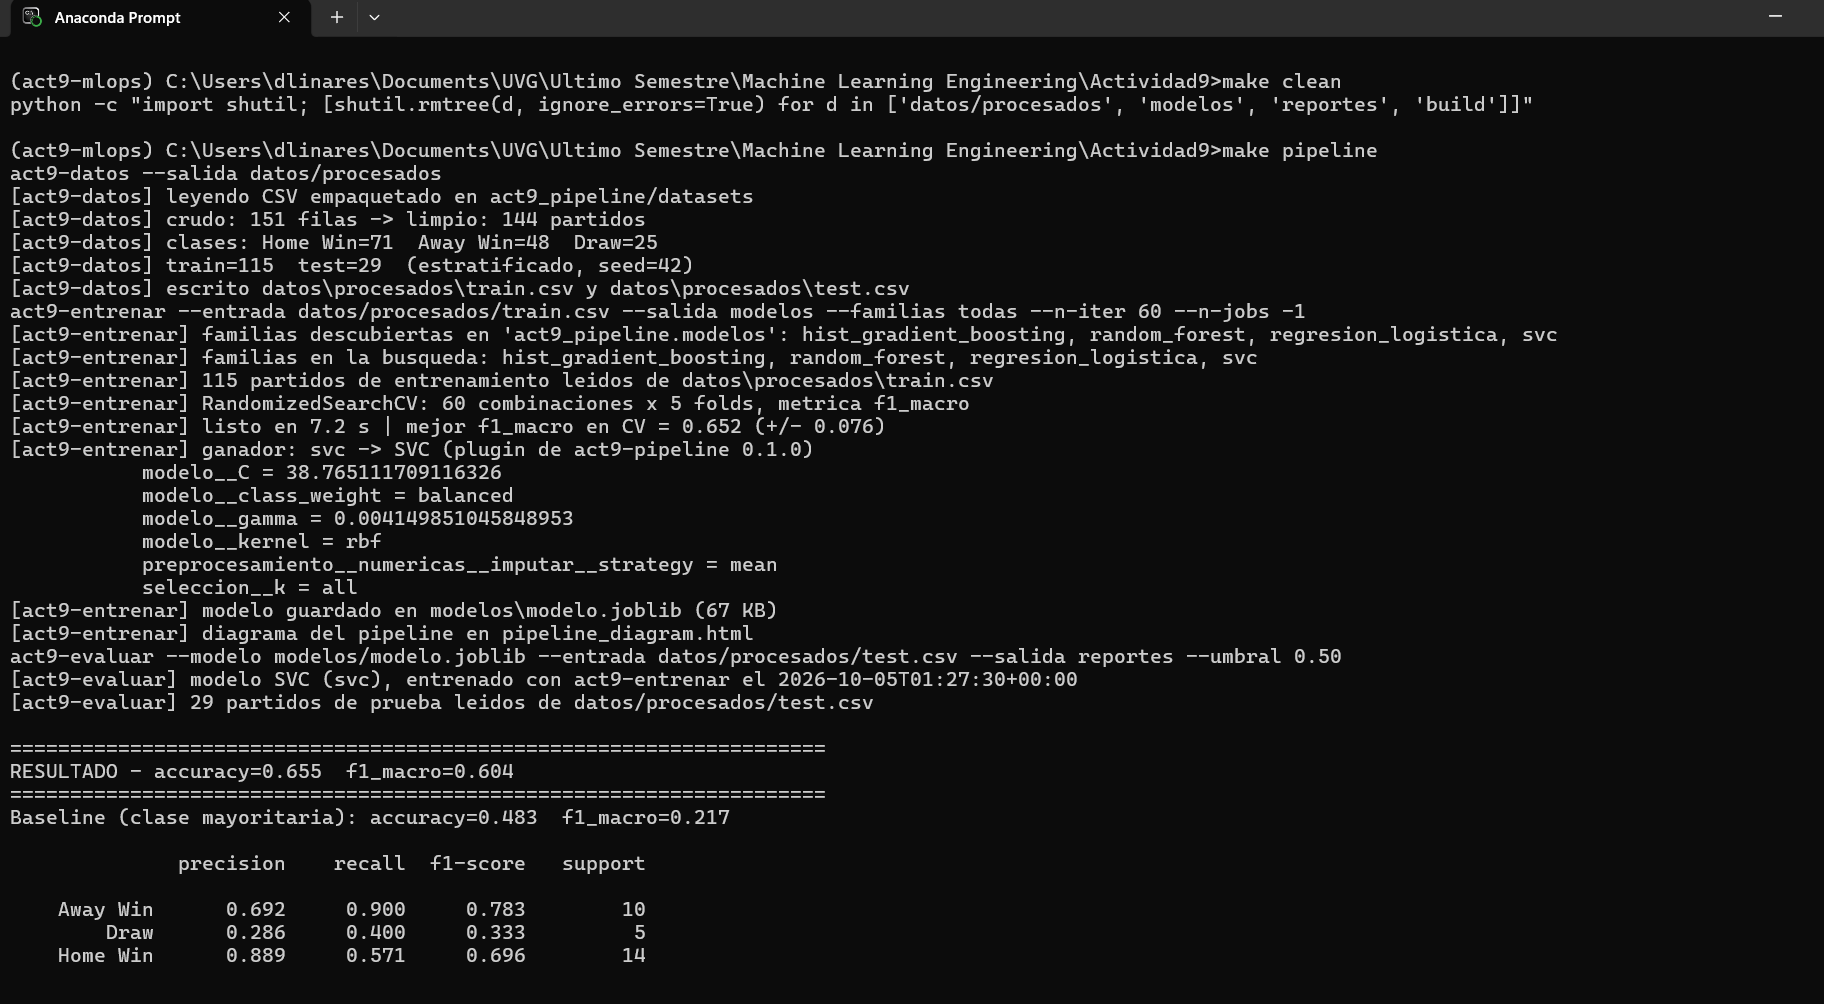
\includegraphics[width=\textwidth]{01-make-pipeline-datos-entrenar.png}
\end{center}

\texttt{act9-evaluar} pasó la compuerta (\texttt{f1\_macro} de 0.604 contra un umbral de 0.50), así
que make siguió con \texttt{act9-predecir}, que acertó 19 de los 29 partidos de prueba (segunda
captura). Son los mismos números que dio el pipeline con uv, con Poetry y en GitHub Actions.

\begin{figure}[htbp]
\centering
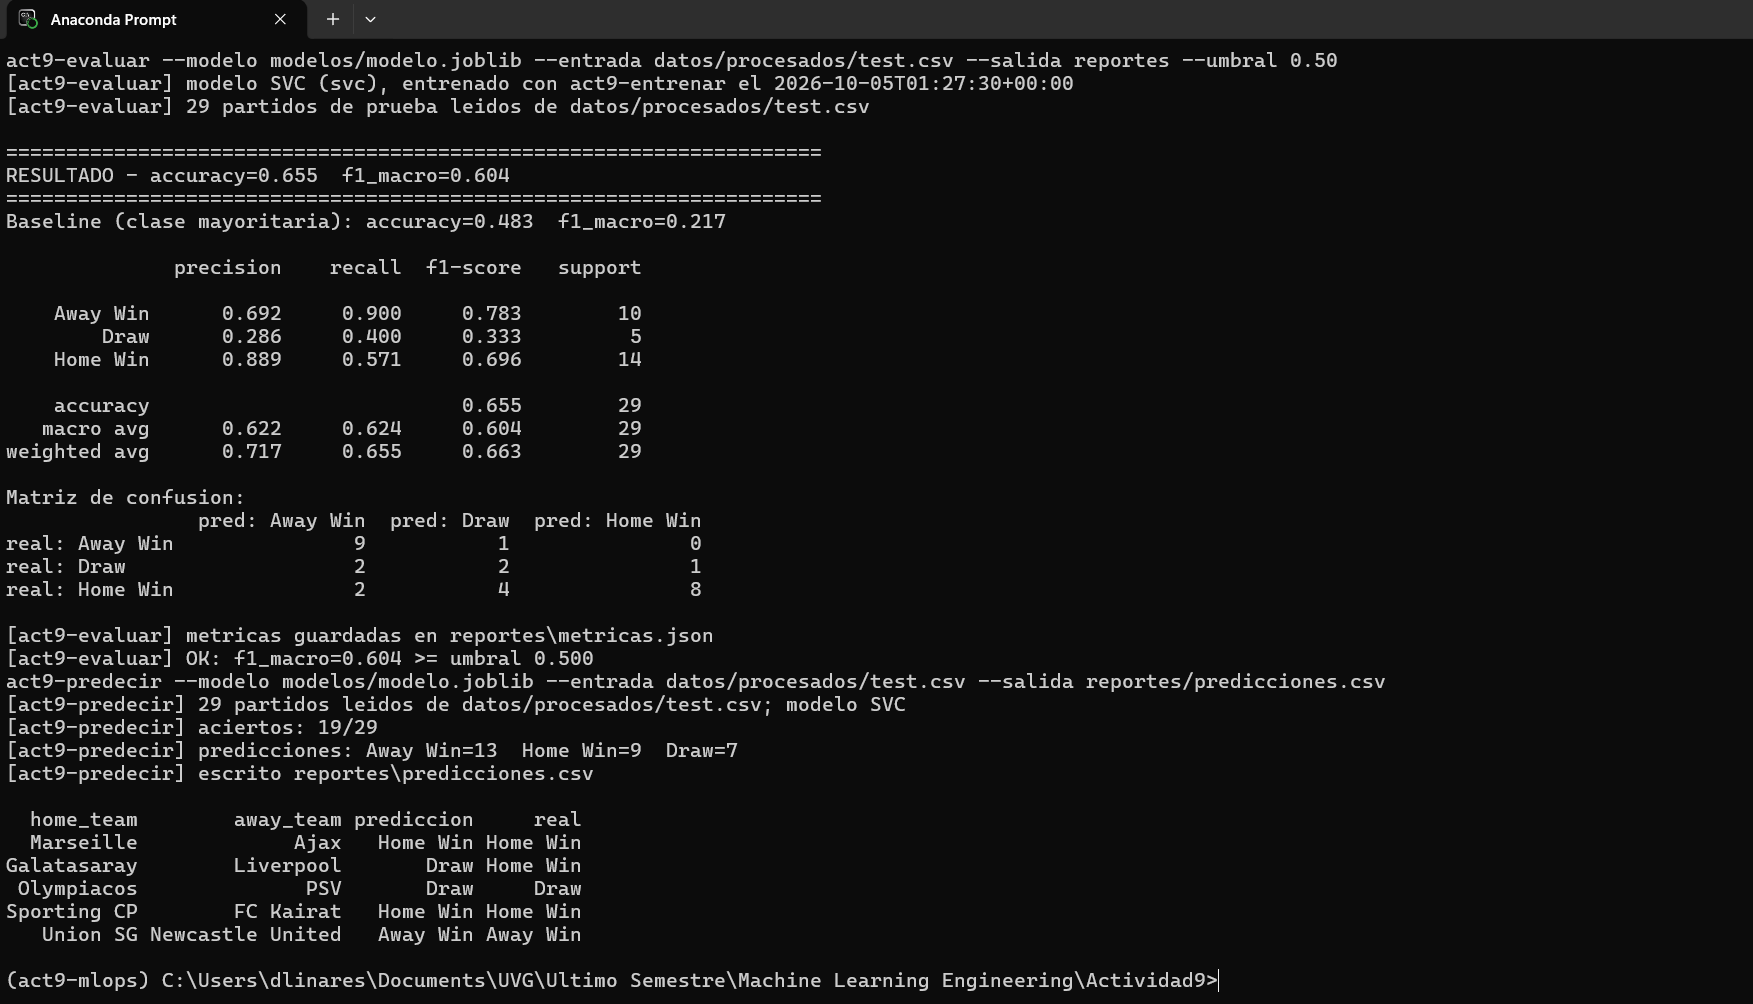
\includegraphics[width=\textwidth]{02-make-pipeline-evaluar-predecir.png}
\end{figure}

\subsection{GitHub Actions}

El workflow de GitHub Actions tiene dos jobs, uno con pip y otro con uv, y ninguno repite comandos
del pipeline:

\begin{verbatim}
- run: make install-dev
- run: make test
- run: make pipeline UMBRAL=0.50
- run: make pipeline RUN="uv run"     # job de uv
\end{verbatim}

Los dos jobs pasaron en el primer intento, en Ubuntu con Python 3.12 (pip) y con el Python que
eligió uv. Entre las pruebas del job de pip está la que exige el 0.619 de la Actividad 3, así que el
resultado también se reproduce en Linux.

% ---------------------------------------------------
\section{Conclusiones}

\begin{enumerate}[leftmargin=1.4em]
\item \textbf{Un entry point es una función con nombre.} Abrir el \texttt{.exe} que generó pip lo
deja claro: importa la función y llama \texttt{sys.exit(main())}. Todo lo demás (dónde queda el
ejecutable, si es \texttt{.exe} o \texttt{.cmd}) lo decide el instalador. Por eso el mismo
\texttt{pyproject.toml} funcionó con pip, conda, uv y Poetry.

\item \textbf{Dividir el pipeline en comandos lo acerca a producción.} Con un solo
\texttt{act3-demo} no se podía predecir sin reentrenar. Con un comando por etapa, cada una se corre,
se programa y se reintenta por separado, y las etapas se comunican por archivos que se pueden
guardar o revisar.

\item \textbf{El código de salida es la parte más útil para MLOps.} Que \texttt{act9-evaluar}
devuelva 1 cuando el modelo no alcanza el umbral permitió que make, y luego GitHub Actions,
detuvieran el pipeline antes de predecir con un modelo malo, sin leer la salida.

\item \textbf{Los plugins dan flexibilidad, pero también variabilidad.} Instalar
\texttt{act9-\allowbreak modelo-\allowbreak knn} agregó una familia sin tocar el pipeline, pero también cambió el resultado
de la búsqueda. Lo que hay instalado en el ambiente pasa a ser parte del modelo, así que en
producción hay que fijar las familias y las versiones de los paquetes.

\item \textbf{El Makefile y el entry point son capas distintas.} El entry point dice qué hace cada
etapa, el Makefile cuándo correrla y GitHub Actions dónde. Cada capa queda corta y legible, y la
misma orden (\texttt{make pipeline}) sirve en Windows, en Linux y en CI.

\item \textbf{En nuestra opinión, lo que más enseñó fue lo que falló.} Los comandos no se
encontraron al no activar el ambiente, make no encontró el \texttt{Makefile} al correrlo desde otra
carpeta, Poetry reemplazó los ejecutables de pip en el mismo \texttt{.venv}, y el notebook volvió a
arrancar con el Python global como en el Taller 2. En los cuatro casos el código estaba bien y el
problema era el ambiente. Por eso \texttt{act9 info} imprime el
intérprete, el gestor y la ruta de cada comando.
\end{enumerate}

% ---------------------------------------------------
\section{Referencias}

\begin{referencias}

\item Astral. (s.f.). \emph{Configuring projects: Entry points}. Documentación de uv.
\url{https://docs.astral.sh/uv/concepts/projects/config/}

\item Awan, A. A. (2024). \emph{GitHub Actions and MakeFile: A hands-on introduction}. DataCamp.
\url{https://www.datacamp.com/tutorial/makefile-github-actions-tutorial}

\item conda-build. (s.f.). \emph{Defining metadata (meta.yaml): Python entry points}.
\url{https://docs.conda.io/projects/conda-build/en/stable/resources/define-metadata.html}

\item Poetry. (s.f.). \emph{The pyproject.toml file}.
\url{https://python-poetry.org/docs/pyproject/}

\item Python Packaging Authority. (s.f.-a). \emph{Entry points specification}.
\url{https://packaging.python.org/en/latest/specifications/entry-points/}

\item Python Packaging Authority. (s.f.-b). \emph{Creating and discovering plugins}.
\url{https://packaging.python.org/en/latest/guides/creating-and-discovering-plugins/}

\end{referencias}

\end{document}
